\documentclass[tikz,border=8pt]{standalone}
\usepackage[scaled=0.95]{helvet}
\renewcommand{\familydefault}{\sfdefault}
\usetikzlibrary{arrows.meta,patterns}
\definecolor{TEJNavy}{HTML}{1E2B55}
\definecolor{TEJBlue}{HTML}{1769AA}
\definecolor{TEJRed}{HTML}{B3261E}
\definecolor{TEJGold}{HTML}{B8860B}
\begin{document}
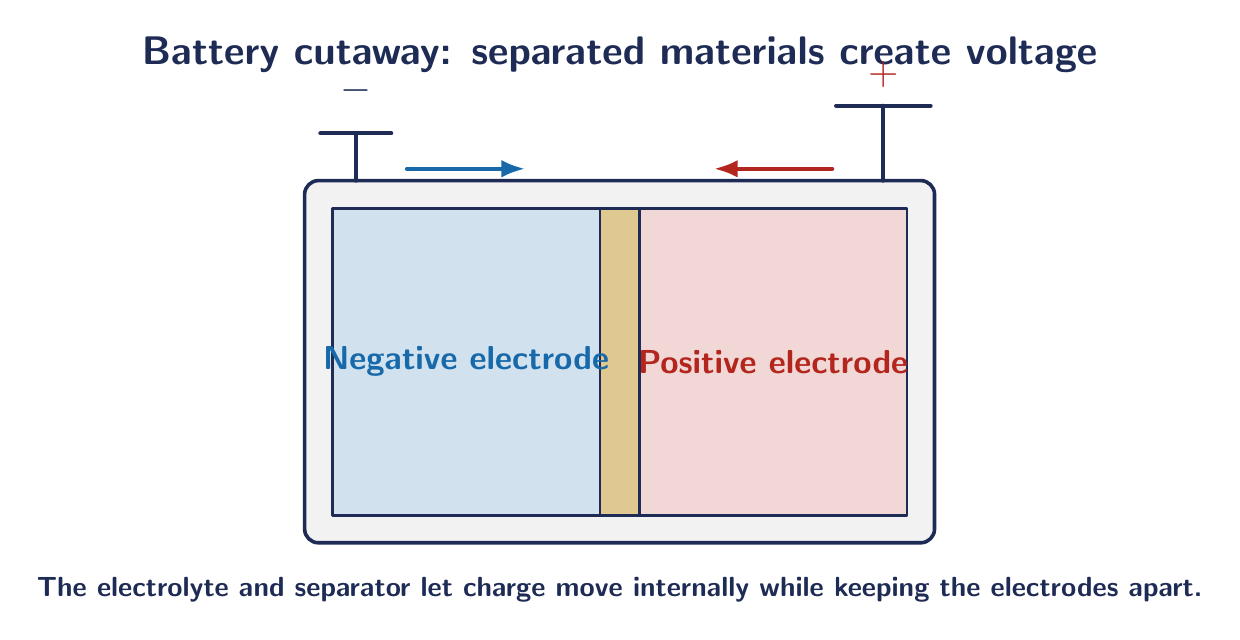
\begin{tikzpicture}[line cap=round,line join=round,font=\sffamily]
  \filldraw[fill=black!5,draw=TEJNavy,line width=1.3pt,rounded corners=5pt] (0,0) rectangle (8,4.6);
  \fill[TEJBlue!20] (0.35,0.35) rectangle (3.75,4.25);
  \fill[TEJRed!18] (4.25,0.35) rectangle (7.65,4.25);
  \filldraw[fill=TEJGold!45,draw=TEJNavy,line width=1pt] (3.75,0.35) rectangle (4.25,4.25);
  \draw[TEJNavy,line width=1pt] (0.35,0.35) rectangle (7.65,4.25);
  \draw[TEJNavy,line width=1.5pt] (0.65,4.6) -- (0.65,5.2);
  \draw[TEJNavy,line width=1.5pt] (0.2,5.2) -- (1.1,5.2);
  \draw[TEJNavy,line width=1.5pt] (7.35,4.6) -- (7.35,5.55);
  \draw[TEJNavy,line width=1.5pt] (6.75,5.55) -- (7.95,5.55);
  \node[font=\bfseries\Large,text=TEJNavy] at (4,6.2) {Battery cutaway: separated materials create voltage};
  \node[font=\bfseries\large,text=TEJBlue] at (2.05,2.3) {Negative electrode};
  \node[font=\bfseries\large,text=TEJRed] at (5.95,2.3) {Positive electrode};
  \node[font=\bfseries,text=TEJNavy,align=center] at (4,-0.6) {The electrolyte and separator let charge move internally while keeping the electrodes apart.};
  \node[font=\bfseries\Large,text=TEJNavy] at (0.65,5.75) {$-$};
  \node[font=\bfseries\Large,text=TEJRed] at (7.35,5.95) {$+$};
  \draw[-{Latex[length=3mm]},TEJRed,line width=1.5pt] (6.7,4.75) -- (5.2,4.75);
  \draw[-{Latex[length=3mm]},TEJBlue,line width=1.5pt] (1.3,4.75) -- (2.8,4.75);
\end{tikzpicture}
\end{document}
